\newcommand{\templatesdir}{../../../templates}
\newcommand{\template}{template-roteiro-est}
\input{\templatesdir/\template/template}

\newcommand{\content}{Complexidade de algoritmos}
\newcommand{\class}{Algoritmos e Estruturas de Dados}
\newcommand{\shortcourse}{45EST}

\begin{document}

\makeheader

{
Leitura obrigatória:
\begin{itemize}
	\item Capítulo 4 de~\cite{GoodrichAndTamassia2013} -- Ferramentas de análise.
\end{itemize}

Leitura complementar:
\begin{itemize}
	\item Capítulo 2 de~\cite{Preiss2001} -- Análise de algoritmos.
	\item Capítulo 3 de~\cite{Preiss2001} -- Notação assintótica.
\end{itemize}
}

\medskip

\newtitle{Conceitos básicos}

Algumas definições:
\begin{itemize}
	\item \textbf{Algoritmo:} sequência de passos para realizar uma tarefa.
	\item \textbf{Estrutura de dados:} forma sistemática de organizar e acessar os dados.
\end{itemize}

\block{
	Como definir se eles são bons?\\%
	Como comparar dois algoritmos ou duas estruturas?%
}

Análise de algoritmos:
\begin{itemize}
	\item Correção / corretude.
	\item Complexidade.
	\begin{itemize}
		\item Tempo de execução.
		\item Consumo de memória.
	\end{itemize}
\end{itemize}

\medskip

%Como demonstrar a \textbf{correção}?
%\begin{itemize}
%	\item Exemplos ou contra-exemplos.
%	\item Contrapositivos ou contradição.
%	\item Indução.
%	\item Invariantes de laço.
%\end{itemize}
%
%\block{As técnicas de prova de algoritmos serão apresentadas adiante.}

Como analisar a \textbf{complexidade}?
\begin{itemize}
	\item Executar o algoritmo e plotar os resultados.
	\begin{itemize}
		\item Sensível às entradas escolhidas.
		\item Comparação prejudicada. \inblock{$\gets$ software, hardware, entradas...}
		\item Necessário implementar e executar todas as opções.
	\end{itemize}
	\item \textbf{Solução:} métodos analíticos.
	\begin{itemize}
		\item Complexidade $\to$ função $f(n)$. \inblock{$\gets n$ é o tamanho da entrada.}
	\end{itemize}
\end{itemize}

\medskip

\underline{Exemplo:}
\begin{itemize}
	\item Algoritmo A possui complexidade $n$.
	\begin{itemize}
		\item Entrada de tamanho $n$ -- tempo máximo de processamento $cn$.
		\begin{itemize}
			\item $c$: constante que modela a variação por hardware e software.
		\end{itemize}
		\item Melhor que um algoritmo B, com complexidade $n^2$.
	\end{itemize}
\end{itemize}


\newtitle{Análise de algoritmos}

Ideia geral:
\begin{itemize}
	\item Contar o número de operações primitivas executadas.
	\item Cada operação primitiva terá um tempo de processamento constante.
	\item Quanto menor o número de operações, melhor o algoritmo.
	
		\item Operações primitivas:
		\begin{itemize}
			\item Atribuição de valores.
			\item Operações aritméticas.
			\item Comparação de valores.
			\item Acesso a uma posição de um vetor.
			\item Recuperar a referência de um objeto.
			\item Chamada de método.
			\item Retorno de um método.
		\end{itemize}
\end{itemize}

\bigskip

\underline{Exemplo:}

\medskip

Algoritmo \texttt{arrayMax(A, n)}:
\begin{minted}{java}
// Entrada: um vetor $A$ com $n \ge 1$ elementos inteiros.
// Saída: o maior elemento de $A$.

@$currentMax \gets A[0]$@
for @$i \gets 1$@ to @$n - 1$@ do
	if @$currentMax < A[i]$@ then
		@$currentMax \gets A[i]$@

return @$currentMax$@
\end{minted}

\medskip

Contando as operações do algoritmo \texttt{arrayMax(A, n)}:

\begin{table}[H]
	\centering
	\small
	\begin{tabular}{c|l}
		Linha & Operações \\
		\hline
		4 & $2$ \\
		5 & $1$ inicialização + $n$ comparações + $2(n - 1)$ incrementos = $3n - 1$ \\
		6 & $2(n - 1) = 2n - 2$ \\
		7 & de $0$ [nunca entra] a $2(n - 1) = 2n - 2$ [entra todas as vezes] \\
		9 & 1
	\end{tabular}
\end{table}

\begin{itemize}
	\item Complexidade no \textbf{melhor caso}: $5n$.
	\item Complexidade no \textbf{pior caso}: $7n - 2$.
	\begin{itemize}
		\color{redtext}
		\item Para qualquer entrada de tamanho $n$, o algoritmo executará no máximo $7n - 2$ operações.
		\item É simples de conduzir/estimar.
		\item Sabe-se que o algoritmo analisado nunca será pior que a estimativa.
	\end{itemize}
\end{itemize}

\medskip

Principais tipos de função de complexidade:
\begin{itemize}
	\item Constante $\to$ $1$
	\item Logarítmica $\to$ $\log n$
	\item Linear $\to$ $n$
	\item n-log-n $\to$ $n \log n$
	\item Quadrática $\to$ $n^2$
	\item Cúbica $\to$ $n^3$
	\item Polinomial $\to$ $n^k$
	\item Exponencial $\to$ $a^n$
\end{itemize}

\medskip

Taxas de crescimento das funções de complexidade:

\begin{figure}[H]
	\centering
	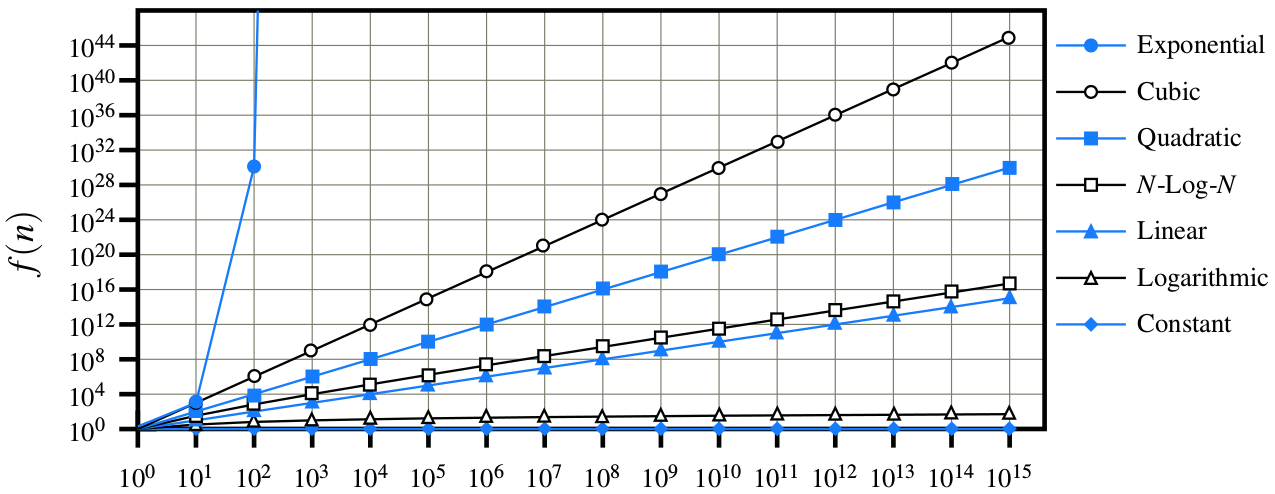
\includegraphics[width=0.79\linewidth]{img/comparacao-funcoes}
\end{figure}

\clearpage

\underline{Exercícios:}
\begin{itemize}
	\item Calcule o número máximo de passos (pior caso) para o algoritmo abaixo.
\end{itemize}

\begin{minted}{java}
for(int i = 0; i < n; i++) {
	for(int j = 0; j < n; j++) {
		if(grade[i][j] != 0) {
			// Operação com complexidade 1
		}
	}
}
\end{minted}

\medskip

{\color{redtext}
\underline{Resposta:}
\begin{itemize}
	\item Laço externo executa $3n + 2$ operações.
	\begin{itemize}
		\item Inicialização ($1$), comparações ($n + 1$) e incremento ($2n$).
	\end{itemize}
	\item Laço interno possui a mesma complexidade, mas é executado $n$ vezes.
	\begin{itemize}
		\item Logo, $n(3n + 2) = 3n^2 + 2n$.
	\end{itemize}
	\item Condicional é executado $n^2$ vezes. Logo, $2n^2$.
	\item Operação é executada $n^2$ vezes, no pior caso.
	\item Resultado: $6n^2 + 5n + 2$.
\end{itemize}
}

\medskip

\newtitle{Análise assintótica}

Problemas da análise completa:
\begin{itemize}
	\item Muito detalhado.
	\item Oneroso. \inblock{$\gets$ ver exemplo do algoritmo \texttt{arrayMax}.}
	\item Pouca precisão. \inblock{$\gets$ não considera baixo nível, hardware...}
\end{itemize}

\clearpage

O que importa:
\begin{itemize}
	\item A \textbf{taxa de crescimento} do tempo de execução em função de $n$.
	\item Para modelar isso, usamos a notação $O$.
\end{itemize}

\medskip

\textbf{Notação $O$}

{\color{redtext}

``\textit{Sejam $f(n)$ e $g(n)$ funções mapeando números inteiros (tamanho da entrada) em reais (tempo de execução). Dizemos que $f(n)$ é $O(g(n))$ se existe uma constante real $c > 0$ e uma constante inteira $n_0 \ge 1$ tais que $f(n) \le cg(n)$ para todo inteiro $n \ge n_0$.}''

Exemplo de relação definida pela notação $O$:

\begin{figure}[H]
	\centering
	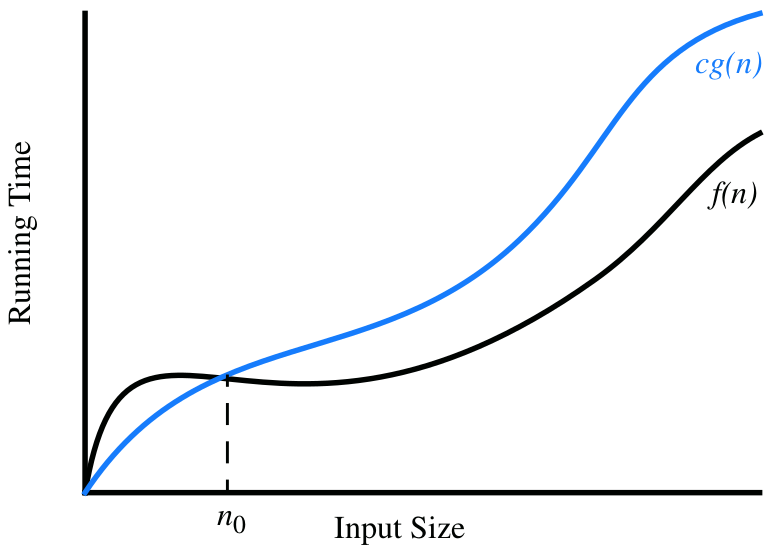
\includegraphics[width=0.55\linewidth]{img/exemplo-o}
\end{figure}

\textbf{Proposição.} A função $7n - 2$ é $O(n)$.

\begin{proof}
Ao escolher $c = 7$ e $n_0 = 1$, temos que $7n - 2 \le cn$, para todo inteiro $n \ge n_0$. Logo, $7n - 2$ é $O(n)$.
\end{proof}

}

\block{Logo, a complexidade do algoritmo \texttt{arrayMax} é $O(n)$, isto é,\\complexidade linear.}

Observações:
\begin{itemize}
	\item A notação $O$ determina que uma função $f(n)$ é ``menor ou igual a'' outra função $g(n)$, descontando-se um fator constante, a medida que $n$ cresce para infinito.
	
	\item Um algoritmo A com complexidade $O(n^2)$ nunca terá um tempo de execução superior a $n^2$, para uma determinada entrada $n$.
\end{itemize}

Regras para definir a complexidade $O$:
\begin{itemize}
	\item Função polinomial: sempre considerar o maior grau.
	\begin{itemize}
		\item $5n^4 + 3n^3 + 2n^2 + 4n + 1$ é $O(n^4)$.
		\item $n^3 + 600n$ é $O(n^3)$.
	\end{itemize}
	
	\item Constantes e multiplicadores são eliminados.
	\begin{itemize}
		\item $2^{n + 2} + 4$ é $O(2^n)$.
		\item $4n^3$ é $O(n^3)$.
	\end{itemize}
	
	\item Função mista: sempre considerar o termo de maior complexidade.
	\begin{itemize}
		\item $5n^2 + 3n \log n + 2n + 5$ é $O(n^2)$.
		\item $3 \log n + 2$ é $O(\log n)$.
		\item $2n + 100 \log n$ é $O(n)$.
	\end{itemize}
	
	\item Sempre considerar a menor complexidade possível para a notação $O$.
	\begin{itemize}
		\item É verdade que $4n^2 + 10$ é $O(n^4)$, mas é melhor dizer que é $O(n^2)$.
	\end{itemize}
	
	\item Sempre considerar a representação mais simples.
	\begin{itemize}
		\item $4n^2 + 2 \log n$ é $O(n^2)$, o que é melhor que $O(n^2 + \log n)$.
	\end{itemize}
\end{itemize}

\clearpage

Outras notações:
\begin{itemize}
	\item Notação $\Omega$: define que a função é maior ou igual a $\Omega(g(n))$.
	\item Notação $\Theta$: define que a função cresce na mesma taxa que $\Theta(g(n))$.
\end{itemize}

\medskip

\newtitle{Comparação}

\textbf{Comparação 1:} crescimento do tempo de execução em função do tamanho da entrada.

\begin{figure}[H]
	\centering
	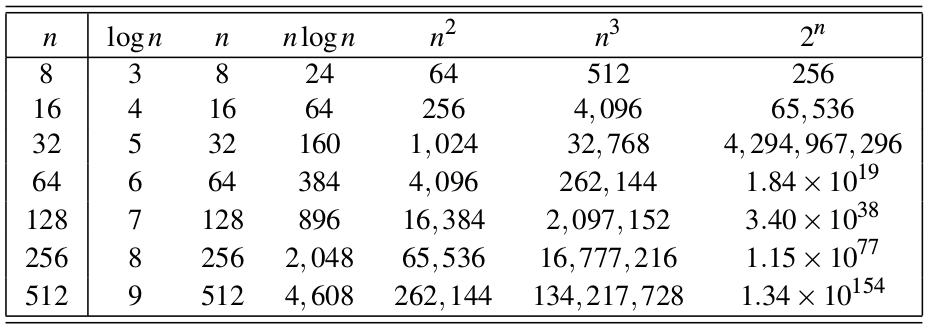
\includegraphics[width=0.7\linewidth]{img/comparacao-complexidade}
\end{figure}

\textbf{Comparação 2:} tamanho máximo do problema que diferentes algoritmos podem resolver em tempos limite distintos.

\begin{figure}[H]
	\centering
	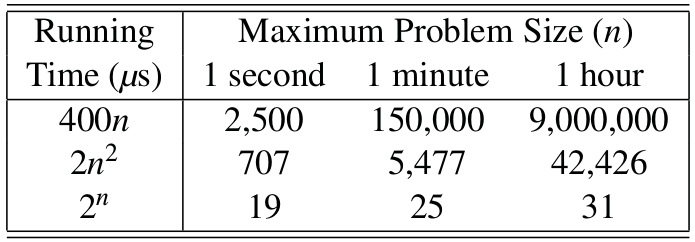
\includegraphics[width=0.4\linewidth]{img/comparacao-tamanhos}
\end{figure}

\textbf{Comparação 3:} aumento no tamanho máximo a ser resolvido usando um computador 256 vezes mais rápido ($m$ é o tamanho máximo da tabela anterior).

\begin{figure}[H]
	\centering
	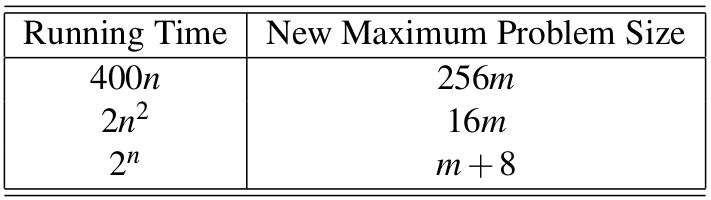
\includegraphics[width=0.4\linewidth]{img/comparacao-speedup}
\end{figure}

\clearpage

\newtitle{Exemplos}

\textbf{Exemplo 1}

Algoritmo \texttt{sumNumbers(n1, n2)}:
\begin{minted}{java}
// Soma dois números inteiros.
public static int sumNumbers(int n1, int n2) {
	int result = n1 + n2;
	return result;
}
\end{minted}

Análise:
\begin{itemize}
	\item Linha 3: 2 operações.
	\item Linha 4: 1 operação.
	\item Complexidade constante: $O(1)$.
	\item Algoritmo de tempo constante.
\end{itemize}

\medskip

\rule{\textwidth}{1pt}

\textbf{Exemplo 2}

Algoritmo \texttt{repeat1(char c, int n)}:
\begin{minted}{java}
// Compõe uma String com o caracter $c$ repetido $n$ vezes.
public static String repeat1(char c, int n) {
	String answer = "";
	for (int j = 0; j < n; j++)
		answer += c;
	return answer;
}
\end{minted}

Análise:
\begin{itemize}
	\item O comando \texttt{answer += c} implica em criar uma nova String, copiar cada caracter da String antiga para ela, e acrescentar o caracter $c$.
	
	\item A cada iteração, a linha 5 executa $k$ operações, sendo $k$ o tamanho da String \texttt{answer}.
	\begin{itemize}
		\item Operações: $\displaystyle\sum_{j = 0}^{n - 1} j = \frac{n(n + 1)}{2}$. Logo, sua complexidade é $O(n^2)$.
	\end{itemize}
	
	\item Linhas 3, 4 e 6 apresentam operações em tempo constante.
	
	\item Complexidade quadrática: $O(n^2)$.
	\item Algoritmo de tempo quadrático.
\end{itemize}

\medskip

\rule{\textwidth}{1pt}

\textbf{Exemplo 3}

Algoritmo \texttt{repeat2(char c, int n)}:
\begin{minted}{java}
// Compõe uma String com o caracter $c$ repetido $n$ vezes.
public static String repeat2(char c, int n) {
	StringBuilder sb = new StringBuilder();
	for (int j = 0; j < n; j++)
		sb.append(c);
	return sb.toString();;
}
\end{minted}

Análise:
\begin{itemize}
	\item O comando \texttt{sb.append(c)} é executado em tempo constante.
	\item Linhas 3, 4 e 6 apresentam operações em tempo constante.
	\item Complexidade linear: $O(n)$.
	\item Algoritmo de tempo linear.
	\item OBS: o algoritmo é o mesmo, o que muda é a estrutura de dados.
\end{itemize}

\clearpage

\textbf{Exemplo 4}

Algoritmo \texttt{disjoint1(int[] vA, int[] vB, int[] vC)}:
\begin{minted}{java}
// Retorna $true$ se não existe nenhum elemento comum nos três grupos.
// Cada vetor possui elementos distintos dentro de si.
public static boolean disjoint1(int[ ] vA, int[ ] vB, int[ ] vC) {
	for (int a : vA)
		for (int b : vB)
			for (int c : vC)
				if ((a == b) && (b == c))
					return false;
	return true;
}
\end{minted}

Análise:
\begin{itemize}
	\item A operação constante da linha 7 é repetida $n \times n \times n = n^3$ vezes.
	\item Complexidade cúbica: $O(n^3)$.
	\item Algoritmo de tempo cúbico.
\end{itemize}

\medskip

\rule{\textwidth}{1pt}

\textbf{Exemplo 5}

Algoritmo \texttt{disjoint2(int[] vA, int[] vB, int[] vC)}:
\begin{minted}{java}
// Retorna $true$ se não existe nenhum elemento comum nos três grupos.
// Cada vetor possui elementos distintos dentro de si.
public static boolean disjoint2(int[ ] vA, int[ ] vB, int[ ] vC) {
	for (int a : vA)
		for (int b : vB)
			if (a == b)
				for (int c : vC)
					if (a == c)
						return false;
	return true;
}
\end{minted}

Análise:
\begin{itemize}
	\item Os laços das linhas 4 e 5 sempre são executados -- $O(n^2)$.
	\item No máximo $n$ pares $(a, b)$ são iguais, portanto o laço da linha 7 é executado no máximo $n$ vezes.
	\item Complexidade $n^2 + n = O(n^2)$.
	\item Algoritmo de tempo quadrático.
\end{itemize}

\medskip

\rule{\textwidth}{1pt}

\textbf{Exemplo 6}

Algoritmo \texttt{unique1(int[] data)}:
\begin{minted}{java}
// Retorna $true$ se não existe elemento duplicado no vetor.
public static boolean unique1(int[ ] data) {
	int n = data.length;
	for (int j = 0; j < n - 1; j++)
		for (int k = j + 1; k < n; k++)
			if (data[j] == data[k])
				return false;
	return true;
}
\end{minted}

Análise:
\begin{itemize}
	\item O laço interno é executado $(n - 1) + (n - 2) + \dots + 2 + 1$ vezes.
	\item Complexidade quadrática $O(n^2)$.
	\item Algoritmo de tempo quadrático.
\end{itemize}

\clearpage

\textbf{Exemplo 7}

Algoritmo \texttt{unique2(int[] data)}:
\begin{minted}{java}
// Retorna $true$ se não existe elemento duplicado no vetor.
// O vetor é ordenado para verificar apenas os pares de elementos.
public static boolean unique2(int[ ] data) {
	int n = data.length;
	Arrays.sort(data);					// Operação $O(n \log n)$
	for (int j = 0; j < n - 1; j++)
		if (data[j] == data[j+1])
			return false;
	return true;
}
\end{minted}

Análise:
\begin{itemize}
	\item O vetor é percorrido apenas uma vez.
	\item Complexidade linear $O(n)$.
	\item Algoritmo de tempo linear.
\end{itemize}

\rule{\textwidth}{1pt}

\textbf{Exemplo 8}

Algoritmo \texttt{prefixAverage1(double[] x)}:
\begin{minted}{java}
// Retorna um vetor onde cada posição $j$ armazena a média dos
// elementos $x[0] \dots x[j]$.
public static double[] prefixAverage1(double[] x) {
	int n = x.length;
	double[ ] a = new double[n];
	for (int j=0; j < n; j++) {
		double total = 0;
		for (int i=0; i <= j; i++)
			total += x[i];
		a[j] = total / (j+1);
	}
	return a;
}
\end{minted}

Análise:
\begin{itemize}
	\item Linhas 4 e 12 são executadas em tempo constante.
	\item Linha 5 executa em tempo $O(n)$.
	\item Os laços (linhas 6 e 8) totalizam $O(n^2)$.
	\item Complexidade quadrática: $O(n^2)$.
	\item Algoritmo de tempo quadrático.
\end{itemize}

\rule{\textwidth}{1pt}

\textbf{Exemplo 9}

Algoritmo \texttt{prefixAverage2(double[] x)}:
\begin{minted}{java}
// Retorna um vetor onde cada posição $j$ armazena a média dos
// elementos $x[0] \dots x[j]$.
public static double[] prefixAverage2(double[] x) {
	int n = x.length;
	double[] a = new double[n];
	double total = 0;
	for (int j=0; j < n; j++) {
		total += x[j];
		a[j] = total / (j+1);
	}
	return a;
}
\end{minted}

Análise:
\begin{itemize}
	\item O laço percorre o vetor uma única vez.
	\item Complexidade linear: $O(n)$.
	\item Algoritmo de tempo linear.
\end{itemize}

\clearpage

\newtitle{Atividades}

\begin{enumerate}
	\item Leia a respeito das sete funções usadas em~\cite{GoodrichAndTamassia2013} e as proposições e provas a respeito das mesmas.
	
	\item Leia a respeito das técnicas de prova de correção de algoritmos apresentadas em~\cite{GoodrichAndTamassia2013}.
	
	\item Analise o tempo de execução do algoritmo \texttt{BinarySum} (Trecho de Código 3.34 de~\cite{GoodrichAndTamassia2013}) usando valores arbitrários para o parâmetro $n$.
	
	\bigskip
	
	\item Faça os seguintes exercícios de~\cite{GoodrichEtAl2014}.
	\begin{itemize}
		
		\item[R-4.1:] Desenhe o gráfico das funções $8n$, $4n \log n$, $2n^2$, $n^3$ e $2^n$ usando uma escala logarítmica para os eixos $x$ e $y$, isto é, se o valor da função $f(n)$ é $y$, desenhe esse ponto com a coordenada $x$ em $\log x$ e a coordenada $y$ em $\log y$.
		
		\item[R-4.2:] O número de operações executadas pelos algoritmos \texttt{A} e \texttt{B} é $8n \log n$ e $2n^2$, respectivamente. Determine $n_0$ tal que \texttt{A} seja melhor que \texttt{B} para $n \ge n_0$.
		
		\item[R-4.3:] O número de operações executadas pelos algoritmos \texttt{A} e \texttt{B} é $40n^2$ e $2n^3$, respectivamente. Determine $n_0$ de maneira que \texttt{A} seja melhor que \texttt{B} para $n \ge n_0$.
		
		\item[R-4.8:] Ordene as funções a seguir por sua taxa assintótica de crescimento.
		\begin{itemize}
			\item $4n \log n + 2n$
			\item $2^{10}$
			\item $2^{\log n}$
			\item $3n + 100 \log n$
			\item $4n$
			\item $2^n$
			\item $n^2 + 10n$
			\item $n^3$
			\item $n \log n$
		\end{itemize}
		
		\item[R-4.9:] Forneça uma caracterização $O$ em termos de $n$ do tempo de execução do algoritmo abaixo.
		
\begin{minted}{java}
/** Returns the sum of the integers in given array. */
public static int example1(int[] arr) {
	int n = arr.length, total = 0;
	for (int j=0; j < n; j++)
		total += arr[j];
	return total;
}
\end{minted}
		
		\item[R-4.10:] Forneça uma caracterização $O$ em termos de $n$ do tempo de execução do algoritmo abaixo.
\begin{minted}{java}
/** Returns the sum of the integers with even index in given array. */
public static int example2(int[] arr) {
	int n = arr.length, total = 0;
	for (int j=0; j < n; j += 2)
		total += arr[j];
	return total;
}
\end{minted}
		
		\item[R-4.11:] Forneça uma caracterização $O$ em termos de $n$ do tempo de execução do algoritmo abaixo.
\begin{minted}{java}
/** Returns the sum of the prefix sums of given array. */
public static int example3(int[ ] arr) {
	int n = arr.length, total = 0;
	for (int j=0; j < n; j++)
		for (int k=0; k <= j; k++)
			total += arr[j];
	return total;
}
\end{minted}

		\item[R-4.12:] Forneça uma caracterização $O$ em termos de $n$ do tempo de execução do algoritmo abaixo.
\begin{minted}{java}
/** Returns the sum of the prefix sums of given array. */
public static int example4(int[ ] arr) {
	int n = arr.length, prefix = 0, total = 0;
	for (int j=0; j < n; j++) {
		prefix += arr[j];
		total += prefix;
	}
	return total;
}
\end{minted}
		
		\item[R-4.13:] Forneça uma caracterização $O$ em termos de $n$ do tempo de execução do algoritmo abaixo.
\begin{minted}{java}
/** Returns the number of times second array stores sum of prefix sums from first. */
public static int example5(int[] first, int[] second) {
	int n = first.length, count = 0;
	for (int i=0; i < n; i++) {
		int total = 0;
		for (int j=0; j < n; j++)
			for (int k=0; k <= j; k++)
				total += first[k];
		if (second[i] == total) count++;
	}
	return count;
}
\end{minted}		

		\item[R-4.28:] Para cada função $f(n)$ e tempo $t$ da tabela a seguir, determine o maior tamanho de $n$ para um problema $P$ que pode ser resolvido em tempo $t$ se o algoritmo para resolver $P$ consome $f(n)$ microssegundos (uma das entradas já foi feita).
		
		\begin{table}[H]
			\centering
			\begin{tabular}{|c|c|c|c|c|}
				\hline\hline
				           &       1 segundo        & 1 hora & 1 mês & 1 século \\ \hline
				 $\log n$  & $\approx 10 ^{300000}$ &        &       &  \\ \hline
				   $n$     &                        &        &       &  \\ \hline
				$n \log n$ &                        &        &       &  \\ \hline
				  $n^2$    &                        &        &       &  \\ \hline
				  $2^n$    &                        &        &       &  \\ \hline\hline
			\end{tabular} 
		\end{table}
		
		\item[R-4.29:] O algoritmo \texttt{A} executa uma computação em tempo $O(\log n)$ para cada entrada de um arranjo de $n$ elementos. Qual o pior caso em relação ao tempo de execução de \texttt{A}?
		
		\item[R-4.30:] Dado um arranjo \texttt{X} de $n$ elementos, o algoritmo \texttt{B} escolhe $\log n$ elementos de \texttt{X}, aleatoriamente, e executa um cálculo em tempo $O(n)$ para cada um. Qual o pior caso em relação ao tempo de execução de \texttt{B}?
		
		\item[R-4.31:] Dado um arranjo \texttt{X} de $n$ elementos inteiros, o algoritmo \texttt{C} executa uma computação em tempo $O(n)$ para cada número par de \texttt{X} e uma computação em tempo $O(\log n)$ para cada elemento ímpar de \texttt{X}. Qual o melhor caso e o pior caso em relação ao tempo de execução de \texttt{C}?
		
		\item[R-4.32:] Dado um arranjo \texttt{X} de $n$ elementos, o algoritmo \texttt{D} chama o algoritmo \texttt{E} para cada elemento \texttt{X[i]}. O algoritmo \texttt{E} executa em tempo $O(i)$ quando é chamado sobre um elemento \texttt{X[i]}. Qual o pior caso em relação ao tempo de execução do algoritmo \texttt{D}?
	
		\item[R-4.34:] Existe uma cidade bem conhecida (que ficará anônima aqui) cujos habitantes têm a reputação de gostarem de uma refeição somente se essa refeição for a melhor que já experimentaram na vida. Caso contrário, eles a odeiam. Assumindo que a qualidade das refeições está distribuída de maneira uniforme ao longo da vida da pessoa, qual o número esperado de habitantes dessa cidade que estão felizes com suas refeições?
	
		\item[P-4.60:] Implemente \texttt{prefixAverage1} e \texttt{prefixAverage2}, e execute uma análise experimental dos seus tempos de execução. Visualize seus tempos de execução como uma função do tamanho da entrada usando um gráfico \textit{di-log}.
		
		\item[P-4.61:] Execute uma análise experimental cuidadosa que compare os tempos relativos de execução dos métodos apresentados nos exercícios R-4.16 a R-4.20.
		
		\item[P-4.62:] Execute uma análise experimental para testar a hipótese de que o método da biblioteca Java, \texttt{java.util.Arrays.sort} executa em um tempo médio $O(n \log n)$.
		
		\item[P-4.63:] Execute uma análise experimental para determinar o maior valor de $n$ para cada um dos dois algoritmos para resolver o problema do elemento único, de maneira que o algoritmo execute em um minuto ou menos.
	\end{itemize}
\end{enumerate}

\medskip

\newtitle{Referências}
\begingroup
	\footnotesize
	\renewcommand{\chapter}[2]{}%
	\bibliographystyle{apalike}
	\bibliography{../referencias}
\endgroup

\end{document}